\documentclass[]{article}
\usepackage[T1]{fontenc}
\usepackage{lmodern}
\usepackage{amssymb,amsmath}
\usepackage{ifxetex,ifluatex}
\usepackage{fixltx2e} % provides \textsubscript
% use upquote if available, for straight quotes in verbatim environments
\IfFileExists{upquote.sty}{\usepackage{upquote}}{}
\ifnum 0\ifxetex 1\fi\ifluatex 1\fi=0 % if pdftex
  \usepackage[utf8]{inputenc}
\else % if luatex or xelatex
  \ifxetex
    \usepackage{mathspec}
    \usepackage{xltxtra,xunicode}
  \else
    \usepackage{fontspec}
  \fi
  \defaultfontfeatures{Mapping=tex-text,Scale=MatchLowercase}
  \newcommand{\euro}{€}
\fi
% use microtype if available
\IfFileExists{microtype.sty}{\usepackage{microtype}}{}
\usepackage{longtable,booktabs}
\usepackage{graphicx}
% Redefine \includegraphics so that, unless explicit options are
% given, the image width will not exceed the width of the page.
% Images get their normal width if they fit onto the page, but
% are scaled down if they would overflow the margins.
\makeatletter
\def\ScaleIfNeeded{%
  \ifdim\Gin@nat@width>\linewidth
    \linewidth
  \else
    \Gin@nat@width
  \fi
}
\makeatother
\let\Oldincludegraphics\includegraphics
{%
 \catcode`\@=11\relax%
 \gdef\includegraphics{\@ifnextchar[{\Oldincludegraphics}{\Oldincludegraphics[width=\ScaleIfNeeded]}}%
}%
\ifxetex
  \usepackage[setpagesize=false, % page size defined by xetex
              unicode=false, % unicode breaks when used with xetex
              xetex]{hyperref}
\else
  \usepackage[unicode=true]{hyperref}
\fi
\hypersetup{breaklinks=true,
            bookmarks=true,
            pdfauthor={},
            pdftitle={},
            colorlinks=true,
            citecolor=blue,
            urlcolor=blue,
            linkcolor=magenta,
            pdfborder={0 0 0}}
\urlstyle{same}  % don't use monospace font for urls
\setlength{\parindent}{0pt}
\setlength{\parskip}{6pt plus 2pt minus 1pt}
\setlength{\emergencystretch}{3em}  % prevent overfull lines
\setcounter{secnumdepth}{5}

\author{}
\date{}

\begin{document}

{
\hypersetup{linkcolor=black}
\setcounter{tocdepth}{3}
\tableofcontents
}
\section{Chapter 1: Using neural nets to recognize handwritten
digits}\label{chapter-1-using-neural-nets-to-recognize-handwritten-digits}

\subsection{Introduction}\label{introduction}

\textbf{Visual pattern recognition} is one of the application of neural
networks. \textbf{Humans are astoundingly good} at making sense of what
our eyes show us. But nearly all that work is done
\textbf{unconsciously.} And so we don't usually appreciate how
\textbf{tough} a problem our visual systems solve.

The \textbf{difficulty of visual pattern recognition} becomes apparent
if you attempt to write a \textbf{computer program to recognize digits.}

\begin{quote}
Simple intuitions about how we recognize shapes - ``a 9 has a loop at
the top, and a vertical stroke in the bottom right'' - turn out to be
\textbf{not so simple to express algorithmically.}
\end{quote}

\begin{quote}
\textbf{Neural networks} approach the problem in \textbf{a different
way.} The idea is to take a \textbf{large number of handwritten digits,}
known as \textbf{training examples,} and then develop a system which can
\textbf{learn from those training examples.} In other words, the neural
network uses the examples to \textbf{automatically infer rules} for
recognizing handwritten digits. Furthermore, by \textbf{increasing the
number of training examples,} the network can \textbf{learn more about
handwriting,} and so \textbf{improve its accuracy.}
\end{quote}

There are just 100 training digits below, perhaps we could \textbf{build
a better handwriting recognizer} by using \textbf{thousands or even
millions or billions of training examples.}

\begin{figure}[htbp]
\centering
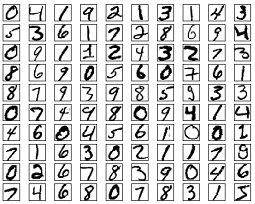
\includegraphics{http://neuralnetworksanddeeplearning.com/images/mnist_100_digits.png}
\caption{100\_handwritten\_digits}
\end{figure}

This chapter is concerned with \textbf{write a computer program
implementing a neural network that learns to recognize handwritten
digits.} The program is \textbf{just 74 lines long,} and uses \textbf{no
special neural network libraries.} But this short program can recognize
digits with an \textbf{accuracy over 96 percent, without human
intervention.} Furthermore, in \textbf{later chapters we'll develop
ideas} which can \textbf{improve accuracy to over 99 percent.}

Focusing on handwriting recognition is an \textbf{excellent prototype}
problem for learning about neural networks in general. As a prototype,
\textbf{it's challenging} but it's \textbf{not so difficult} as to
require an extremely complicated solution, or tremendous computational
power. Furthermore, it's a great way to \textbf{develop more advanced
techniques,} such as \textbf{deep learning.} Later in the book, there
are some discussions about how these ideas may be applied to other
problems in \textbf{computer vision, natural language processing, and
other domains.}

Along the way there are many key ideas about neural networks, including
two important types of artificial neuron \textbf{(the perceptron and the
sigmoid neuron),} and the \textbf{standard learning algorithm} for
neural networks, known as \textbf{stochastic gradient descent.}

\subsection{Perceptrons}\label{perceptrons}

\textbf{Perceptron is a type of artificial neuron.} Perceptrons were
\textbf{developed in the 1950s and 1960s} by the scientist \textbf{Frank
Rosenblatt,} inspired by \textbf{earlier work by Warren McCulloch and
Walter Pitts.} \textbf{Today, it's more common to use other models} of
artificial neurons - in this book, and in much modern work on neural
networks, the \textbf{main neuron model used is one called the sigmoid
neuron.}

A perceptron takes several \textbf{binary inputs,} \$ x\_1, x\_2,
\ldots{}, \$ and produces a single binary output:

\begin{figure}[htbp]
\centering
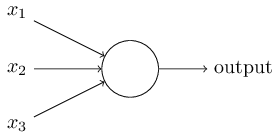
\includegraphics{http://neuralnetworksanddeeplearning.com/images/tikz0.png}
\caption{binary\_inputs}
\end{figure}

In general it could have \textbf{more or fewer inputs.} Rosenblatt
proposed a simple rule to compute the output. He introduced
\textbf{weights, w1,w2,\ldots{}, real numbers} expressing the
\textbf{importance of the respective inputs to the output.} The
\textbf{neuron's output, 0 or 1,} is determined by whether the
\textbf{weighted sum} $\sum_j w_jx_j $ is \textbf{less than or greater
than some threshold value.} Just like the weights, the \textbf{threshold
is a real number} which is a \textbf{parameter of the neuron.} To put it
in more precise algebraic terms:

\begin{equation}  
    output =  
    \begin{cases}
        0,& if \hspace{0.5 cm} \sum_j\ w_jx_j \leqslant threshold \\
        1,& if \hspace{0.5 cm} \sum_j\ w_jx_j > threshold 
    \end{cases}
\end{equation}

That's all there is to how a perceptron works!

That's the \textbf{basic mathematical model.} A way you can think about
the perceptron is that it's a device that \textbf{makes decisions by
weighing up evidence.}

\begin{quote}
Suppose the weekend is coming up, and you've heard that there's going to
be a cheese festival in your city. You like cheese, and are trying to
decide whether or not to go to the festival. You might make your
decision by \textbf{weighing up three factors:} 1. Is the weather good?
2. Does your boyfriend or girlfriend want to accompany you? 3. Is the
festival near public transit? (You don't own a car). We can represent
these three factors by corresponding \textbf{binary variables \$ x\_1,
x\_2 \$ and \$ x\_3. $** For instance, we'd have $ x\_1 = 1 \$ if the
}weather is good,** and \$ x\_1 = 0 \$ if the \textbf{weather is bad.}
Similarly, \$ x\_2 = 1 \$ if \textbf{your boyfriend or girlfriend wants
to go,} and \$ x\_2 = 0 \$ if \textbf{not.} And similarly again for \$
x\_3 \$ and public transit. Now, suppose \textbf{you absolutely adore
cheese,} so much so that you're happy to go to the festival \textbf{even
if your boyfriend or girlfriend is uninterested} and the
\textbf{festival is hard to get to.} But perhaps there's \textbf{no way
you'd go to the festival if the weather is bad.} You can use perceptrons
to model this kind of \textbf{decision-making.} One way to do this is to
\textbf{choose a weight \$ w\_1 = 6 \$ for the weather,} and \$ w\_2 = 2
\$ and \$ w\_3 = 2 \$ for the other conditions. The \textbf{larger value
of w1 indicates that the weather matters a lot to you.} Finally, suppose
you choose a \textbf{threshold of 5} for the perceptron. With these
choices, the perceptron implements the desired decision-making model,
\textbf{outputting 1 whenever the weather is good, and 0 whenever the
weather is bad.} It makes no difference to the output whether your
boyfriend or girlfriend wants to go, or whether public transit is
nearby.
\end{quote}

Obviously, the \textbf{perceptron isn't a complete model of human
decision-making!} But what the example illustrates is how a perceptron
can weigh up different kinds of evidence in order to make decisions. And
it should seem plausible that a \textbf{complex network of perceptrons
could make quite subtle decisions:}

\begin{figure}[htbp]
\centering
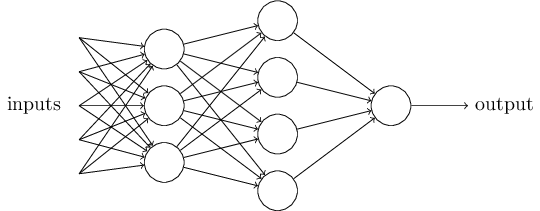
\includegraphics{http://neuralnetworksanddeeplearning.com/images/tikz1.png}
\caption{complex\_network}
\end{figure}

In this network, the first column of perceptrons \textbf{- the first
layer of perceptrons -} is making three very simple decisions, by
weighing the input evidence. What about the perceptrons in the second
layer? Each of those perceptrons is making a decision by weighing up the
results from the first layer of decision-making. In this way a
perceptron in the \textbf{second layer can make a decision at a more
complex and more abstract level than perceptrons in the first layer.}
And even more complex decisions can be made by the perceptron in the
third layer. In this way, a \textbf{many-layer network of perceptrons
can engage in sophisticated decision making.}

In the first example, it is defined perceptrons has just a single
output. \textbf{In the network above the perceptrons look like they have
multiple outputs.} In fact, \textbf{they're still single output.} The
multiple output arrows are merely a useful way of \textbf{indicating
that the output from a perceptron is being used as the input to several
other perceptrons.} It's less unwieldy than drawing a single output line
which then splits.

Let's simplify the way we describe perceptrons. The first change is to
write \$ \sum\emph{j w}jx\_j \$ as a dot product, \$ w⋅x
\equiv \sum\emph{j w}jx\_j
$, where **w and x are vectors whose components are the weights and inputs, respectively.** The second change is to **move the threshold to the other side of the inequality,** and to **replace it by what's known as the perceptron's bias,** $
b \equiv −threshold. \$ Using the bias instead of the threshold, the
perceptron rule can be rewritten:

\begin{equation}
    output =  
    \begin{cases}
        0,& if  \hspace{0.5 cm} w . x + b \leq 0 \\
        1,& if  \hspace{0.5 cm}  w . x + b > 0 
    \end{cases}
\end{equation}

You can think of the \textbf{bias as a measure of how easy it is to get
the perceptron to output a 1.} Or to put it in \textbf{more biological
terms, the bias is a measure of how easy it is to get the perceptron to
fire.} For a perceptron with a \textbf{really big bias, it's extremely
easy for the perceptron to output a 1.} But if the \textbf{bias is very
negative, then it's difficult for the perceptron to output a 1.}

Another way perceptrons can be used is to \textbf{compute the elementary
logical functions} such as \textbf{AND, OR,} and \textbf{NAND.} For
example, suppose we have a perceptron with two inputs, each with weight
−2, and an overall bias of 3. Here's our perceptron:

\begin{figure}[htbp]
\centering
\includegraphics{http://neuralnetworksanddeeplearning.com/images/tikz2.png}
\caption{logical\_perceptron}
\end{figure}

\begin{longtable}[c]{@{}cccl@{}}
\toprule\addlinespace
input 1 & input 2 & output &
\\\addlinespace
\midrule\endhead
0 & 0 & 1 & \$ -2 . 0 -2 . 0 + 3 = 3 \textgreater{} 0 \$
\\\addlinespace
0 & 1 & 1 & \$ -2 . 0 -2 . 1 + 3 = 1 \textgreater{} 0 \$
\\\addlinespace
1 & 0 & 1 & \$ -2 . 1 -2 . 0 + 3 = 1 \textgreater{} 0 \$
\\\addlinespace
1 & 1 & 0 & \$ -2 . 1 -2 . 1 + 3 = -1 \textless{} 0 \$
\\\addlinespace
\bottomrule
\end{longtable}

Our perceptron implements a \textbf{NAND gate!}

The NAND example shows that \textbf{we can use networks of perceptrons
to compute any logical function at all.} The reason is that the
\textbf{NAND gate is universal for computation,} that is, we can build
\textbf{any computation up out of
\href{https://en.wikipedia.org/wiki/NAND_logic}{NAND gates}}. That
means, also \textbf{perceptrons are universal for computation.}

Up to now it is been drawing inputs like \$ x\_1 \$ and \$ x\_2 \$ as
variables floating to the left of the network of perceptrons. In fact,
it's conventional to draw an extra layer of perceptrons - the input
layer - to encode the inputs:

\begin{figure}[htbp]
\centering
\includegraphics{http://neuralnetworksanddeeplearning.com/images/tikz7.png}
\caption{input\_neurons}
\end{figure}

It \textbf{doesn't mean a perceptron with no inputs.} To see this,
suppose we did have a perceptron with no inputs. Then the weighted sum
\$ \sum\emph{j w}jx\_j \$ \textbf{would always be zero,} and so the
perceptron would output \$ 1 \$ if \$ b \textgreater{} 0 $, and $ 0 \$
if \$ b \leq 0
$. That is, the perceptron would simply output a **fixed value, not the desired valued**. It's **better to think of the input perceptrons as not really being perceptrons at all, but rather special units which are simply defined to output the desired values,** $
x\_1, x\_2, \ldots{} \$

\subsection{Sigmoid neurons}\label{sigmoid-neurons}

Suppose we have a network of perceptrons that we'd like to use to learn
to solve some problem. For example, the inputs to the network might be
the raw pixel data from a scanned, handwritten image of a digit. And
we'd like the network to \textbf{learn weights and biases} so that the
\textbf{output from the network correctly classifies the digit.} To see
how learning might work, suppose we \textbf{make a \emph{small change}
in some weight (or bias)} in the network. What we'd like is for this
small change in weight to \textbf{cause only a small corresponding
change in the output} from the network. As we'll see in a moment, this
property will make learning possible. Schematically, here's what we want
(obviously this network is too simple to do handwriting recognition!):

\begin{figure}[htbp]
\centering
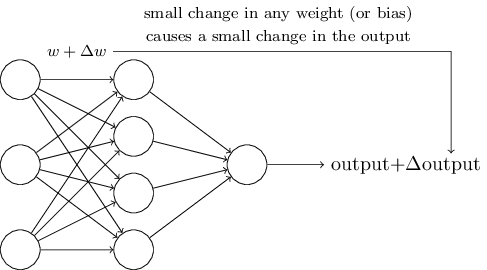
\includegraphics{http://neuralnetworksanddeeplearning.com/images/tikz8.png}
\caption{weight\_small\_change}
\end{figure}

If it were true that a \textbf{small change in a weight (or bias) causes
only a small change in output,} then we could \textbf{use this fact to
modify the weights and biases to get our network to behave more in the
manner we want.}

\begin{quote}
For example, suppose the network was \textbf{mistakenly classifying an
image as an ``8'' when it should be a ``9''.} We could figure out how to
\textbf{make a small change in the weights and biases so the network
gets a little closer to classifying the image as a ``9''.} And then we'd
repeat this, \textbf{changing the weights and biases \emph{over and
over} to produce \emph{better and better} output.} The network would be
learning.
\end{quote}

The problem is that this \textbf{isn't what happens when our network
contains perceptrons.} In fact, a small change in the weights or bias of
any single perceptron in the network can sometimes \textbf{cause the
output of that perceptron to completely flip, say from 0 to 1.} That
flip may then \textbf{cause the behaviour of the rest of the network to
completely change in some very complicated way.}

We can \textbf{overcome this problem} by introducing a new type of
artificial neuron called a \textbf{sigmoid neuron.} Sigmoid neurons are
similar to perceptrons, but \textbf{modified so that small changes in
their weights and bias cause only a small change in their output.}
That's the crucial fact which will allow a network of sigmoid neurons to
learn.

Okay, let me describe the sigmoid neuron. We'll depict sigmoid neurons
in the \textbf{same way we depicted perceptrons.} Just like a
perceptron, the \textbf{sigmoid neuron has inputs,} \$ x\_1, x\_2,
\ldots{} \$ But \textbf{instead of being just 0 or 1,} these inputs can
also \textbf{take on \emph{any values between 0 and 1.}} So, \textbf{for
instance, 0.638\ldots{} is a valid input} for a sigmoid neuron. Also
just like a perceptron, the \textbf{sigmoid neuron has weights} for each
input, \$ w\_1, w\_2, \ldots{} \$ and an \textbf{overall bias,} \$ b
$. But the **output is not 0 or 1.** Instead, it's $ \sigma (w⋅x + b)
$, where $ \sigma \$ is called the \textbf{\emph{sigmoid function}} -
sometimes called \textbf{\emph{logistic function}} - and this new class
of neurons called \textbf{\emph{sigmoid neurons}} or
\textbf{\emph{logistic neurons.}} and is defined by:

\begin{equation}
    \sigma(z) \equiv \frac{1}{1 + e^{-z}}
\end{equation}

The \textbf{output} of a sigmoid neuron with inputs \$ x\_1, x\_2,
\ldots{} \$ weights \$ w\_1, w\_2, \ldots{} \$ and bias \$ b \$ is

\begin{equation}
    \frac {1}{1+exp(−\sum_j w_jx_j − b)}
\end{equation}

To understand the \textbf{similarity} to the perceptron model, suppose
\$ z \equiv w ⋅ x + b \$ is a \textbf{large positive number.} Then \$ e
\^{} \{−z\} \approx 0 \$ and so \$ \sigma(z) \approx 1 \$ just as it
would have been for a perceptron. Suppose on the other hand that \$ z =
w ⋅ x + b \$ is \textbf{very negative.} Then \$ e \^{} \{−z\}
\to \infty $, and $ \sigma(z) \approx 0 \$ like a perceptron. The shape
is:

\begin{figure}[htbp]
\centering
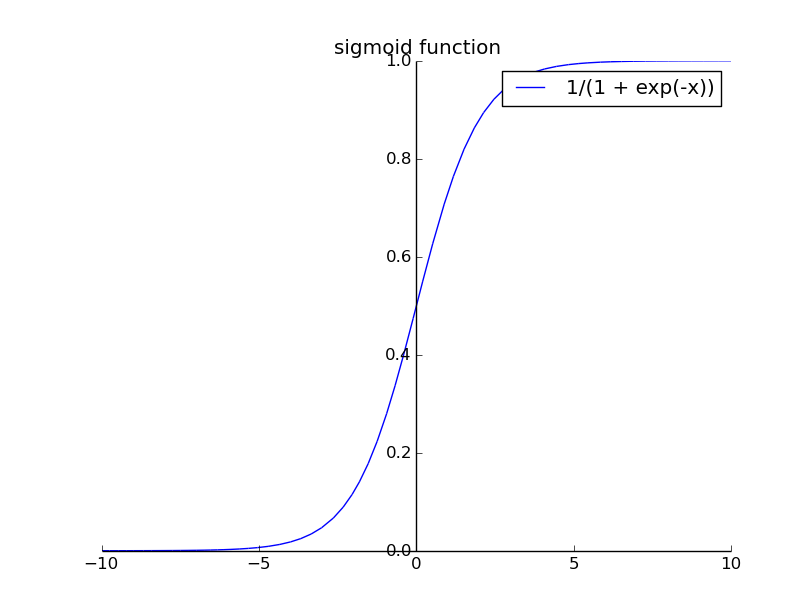
\includegraphics{https://lh3.googleusercontent.com/-WNMDpgwcC7I/VYk-QEgs9DI/AAAAAAAAAT8/MKuAMcVDYcM/s0/sigmoid_function.png}
\caption{sigmoid\_function}
\end{figure}

This shape is a smoothed out version of a \textbf{\emph{step function}}
or \textbf{\emph{Heaviside step function}}:

\begin{figure}[htbp]
\centering
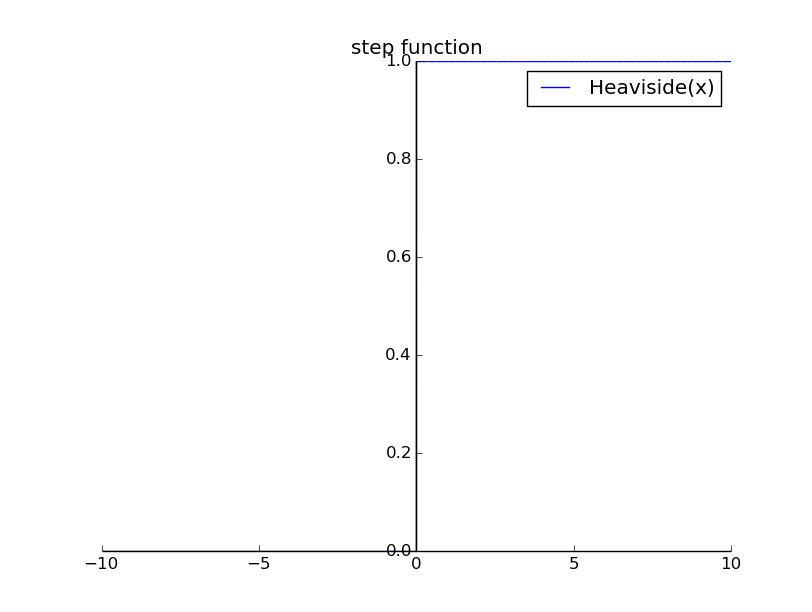
\includegraphics{https://lh3.googleusercontent.com/-lIMAxDaKs5U/VYlCQHeg_1I/AAAAAAAAAUM/gQwIY5OWpAo/s0/step_function.png}
\caption{step\_function}
\end{figure}

If \$ \sigma \$ had in fact been a step function, then the sigmoid
neuron would be a perceptron, since the output would be 1 or 0 depending
on whether \$ w ⋅ x + b \$ was positive or negative. Actually, when \$ w
⋅ x + b = 0 \$ the perceptron outputs 0, while the step function outputs
1. So, strictly speaking, we would need to \textbf{modify the step
function} at that one point.

By using the actual \$ \sigma \$ function we get, a smoothed out
perceptron. The smoothness of \$ \sigma \$ means that small changes \$
\Delta w\_j \$ in the weights and \$ \Delta b \$ in the bias will
produce a small change \$ \Delta output \$ in the output from the
neuron. In fact, calculus tells us that \$ \Delta output \$ is well
approximated by

\begin{equation}
    \Delta output \approx \sum_j 
    \frac {\partial \ output}{\partial w_j} \Delta w_j + 
    \frac {\partial \ output}{\partial b} \Delta b
\end{equation}

where the \textbf{sum is over all the weights,} \$ w\_j $, and $
\frac{\partial \ output}{\partial w_j} \$ and \$
\frac{\partial \ output}{\partial b} \$ denote \textbf{\emph{partial
derivatives}} of the output with respect to \$ w\_j \$ and \$ b \$,
respectively. So while sigmoid neurons have much of the \textbf{same
qualitative behaviour as perceptrons,} they make it \textbf{much easier
to figure out how changing the weights and biases will change the
output.}

If it's the shape of \$ \sigma \$ which really matters, and not its
exact form, then why use the particular form used for \$ \sigma \$ ? In
fact, there are \textbf{other activation functions} as well. The main
thing that changes when we use a different activation function is that
the \textbf{particular values for the partial derivatives in Equation
(5) change.} It turns out that when we compute those partial
derivatives, using \$ \sigma \$ will simplify the algebra.

\begin{equation}
    \begin{split}       
        \frac{d\sigma}{dz} &= \left({1 - \frac{1}{1 + e ^ {-z}}}\right)
        \left(\frac{1}{1 + e ^ {-z}}\right)\\
        &=(1 - \sigma)\sigma
\end{split}
\end{equation}

\begin{quote}
Obviously, one big difference between perceptrons and sigmoid neurons is
that sigmoid neurons don't just output 0 or 1. They can have as output
\textbf{any real number between 0 and 1, so values such as 0.173\ldots{}
and 0.689\ldots{}} are legitimate outputs. This can be useful, for
example, if we want to use the output value to represent the
\textbf{average intensity of the pixels} in an image input to a neural
network. But sometimes it can be a nuisance. Suppose we want the output
from the network to indicate either \textbf{``the input image is a 9''}
or \textbf{``the input image is not a 9''.} Obviously, it would be
easiest to do this if the output was a 0 or a 1, as in a perceptron. But
in practice we can set up a convention to deal with this, for example,
by \textbf{deciding to interpret any output of at least 0.5 as
indicating a ``9'', and any output less than 0.5 as indicating ``not a
9''.}
\end{quote}

\subsection{The architecture of neural
networks}\label{the-architecture-of-neural-networks}

Suppose we have the network:

\begin{figure}[htbp]
\centering
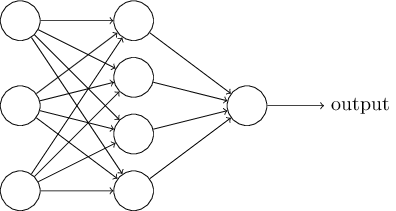
\includegraphics{http://neuralnetworksanddeeplearning.com/images/tikz10.png}
\caption{architecture}
\end{figure}

As mentioned earlier, the \textbf{leftmost layer} in this network is
called the \textbf{\emph{input layer,}} and the neurons within the layer
are called \textbf{\emph{input neurons.}} The \textbf{rightmost or
output layer} contains the \textbf{\emph{output neurons,}} or, as in
this case, a \textbf{single output neuron.} The middle layer is called a
\textbf{\emph{hidden layer,}} since the neurons in this layer are
neither inputs nor outputs. The network above has just a single hidden
layer, but \textbf{some networks have multiple hidden layers.} For
example, the following four-layer network has two hidden layers:

\begin{figure}[htbp]
\centering
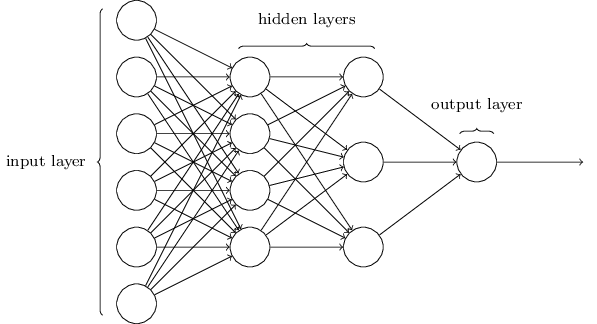
\includegraphics{http://neuralnetworksanddeeplearning.com/images/tikz11.png}
\caption{two\_hidden\_layers}
\end{figure}

Somewhat confusingly, and for historical reasons, \textbf{such multiple
layer networks are sometimes called multilayer perceptrons or MLPs,
despite being made up of sigmoid neurons, not perceptrons.} It is not
going to be used the MLP terminology in this book, since it is
confusing.

\begin{quote}
The \textbf{design of the input and output layers in a network is often
straightforward.} For example, suppose we're trying to determine whether
a handwritten image depicts a ``9'' or not. A natural way to design the
network is to \textbf{encode the intensities of the image pixels into
the input neurons.} If the image is a 64 by 64 grayscale image, then
we'd have \textbf{\$ 4,096 = 64 \times 64 \$ input neurons,} with the
intensities scaled appropriately between 0 and 1. The \textbf{output
layer will contain just a single neuron,} with output values of less
than 0.5 indicating \textbf{``input image is not a 9'',} and values
greater than 0.5 indicating \textbf{``input image is a 9 .''}
\end{quote}

There can be quite an art to the \textbf{design of the hidden layers.}
Neural networks researchers have developed \textbf{many design
heuristics for the hidden layers,} which help people get the behaviour
they want out of their nets. For example, such heuristics can be used to
help determine how to \textbf{trade off the number of hidden layers
against the time required to train the network.}

Up to now, we've been discussing neural networks where the
\textbf{output from one layer is used as input to the next layer.} Such
networks are called \textbf{\emph{feedforward neural networks.}} This
means there are \textbf{no loops} in the network \textbf{- no
feedback-}. Loops would be problematic in for example sigmoid neurons
because of the \textbf{inputs would depend on the outputs.} However,
there are \textbf{other models} of artificial neural networks in which
\textbf{feedback loops are possible.} These models are called
\textbf{\emph{recurrent neural networks.}} The idea in these models is
to have neurons which \textbf{fire for some limited duration of time,
before becoming quiescent.} That \textbf{firing can stimulate other
neurons,} which may fire a little while later, also for a limited
duration. That causes still more neurons to fire, and so over time we
get a \textbf{cascade of neurons firing.} \textbf{Loops don't cause
problems} in such a model, since a \textbf{neuron's output only affects
its input at some later time,} not instantaneously.

Recurrent neural nets have been \textbf{less influential than
feedforward networks,} in part because the \textbf{learning algorithms
for recurrent nets are (at least to date) less powerful.} But recurrent
networks are still extremely interesting. They're much closer in spirit
to \textbf{how our brains work} than feedforward networks. And
\textbf{it's possible that recurrent networks can solve important
problems which can only be solved with great difficulty by feedforward
networks.}

\subsection{A simple network to classify handwritten
digits}\label{a-simple-network-to-classify-handwritten-digits}

We can split the problem of recognizing handwritten digits into two
sub-problems. First, we'd like a way of breaking an image containing
many digits into a sequence of separate images, \textbf{each containing
a single digit.}

\begin{figure}[htbp]
\centering
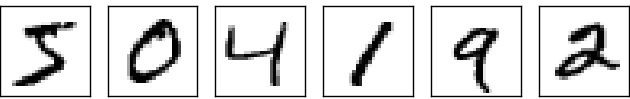
\includegraphics{http://neuralnetworksanddeeplearning.com/images/digits_separate.png}
\caption{digits\_sequence}
\end{figure}

Once the image has been segmented, the program then needs to
\textbf{classify each individual digit.} We will focus on writing a
program to \textbf{classify individual digits.}.

To recognize individual digits we will use a three-layer neural network:

\begin{figure}[htbp]
\centering
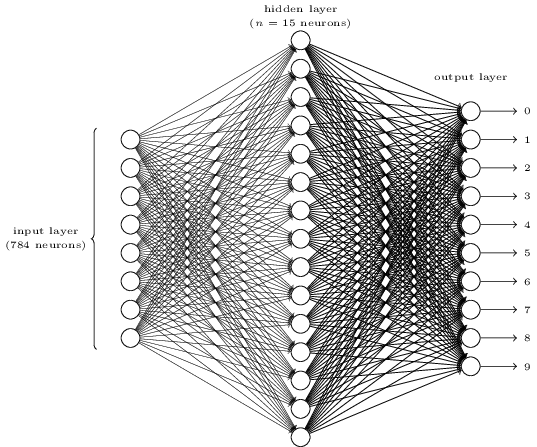
\includegraphics{http://neuralnetworksanddeeplearning.com/images/tikz12.png}
\caption{three\_layer\_neural\_net}
\end{figure}

As discussed in the next section, our training data for the network will
consist of many 28 by 28 pixel images of scanned handwritten digts, and
so the input layer contains \$ 784 = 28 \times 28 \$ neurons. The
\textbf{input pixels are grayscale,} with a value of \textbf{0.0
representing white,} a value of \textbf{1.0 representing black,} and in
between values representing gradually darkening shades of grey.

The second layer of the network is a hidden layer. We denote the
\textbf{number of neurons in this hidden layer by n,} and we'll
\textbf{experiment with different values for n.}

\begin{quote}
The \textbf{output layer of the network contains 10 neurons.} If the
first neuron fires, i.e., has an \$ output \approx  1 \$, then that will
indicate that the network thinks the digit is a 0. If the second neuron
fires then that will indicate that the network thinks the digit is a 1.
And so on. A little more precisely, we number the \textbf{output neurons
from 0 through 9,} and figure out \textbf{which neuron has the highest
activation value.} If that neuron is, say, neuron number 6, then our
network will guess that the input digit was a 6. And so on for the other
output neurons.
\end{quote}

Why we use 10 output neurons. After all, the goal of the network is to
tell us which digit \$ (0, 1, 2, \ldots{}, 9) \$ corresponds to the
input image. A seemingly natural way of doing that is to use
\textbf{just 4 output neurons,} treating \textbf{each neuron as taking
on a binary value,} depending on whether the neuron's output is closer
to 0 or to 1. Four neurons are enough to encode the answer, since \$ 2
\^{} 4 = 16 \$ is more than 10 possible values for the input digit.
\textbf{Why should our network use 10 neurons instead? } The ultimate
\textbf{justification is empirical.} We can \textbf{try out both network
designs,} and it turns out that, \textbf{for this particular problem,
the network with 10 output neurons learns to recognize digits better
than the network with 4 output neurons.} But that leaves us wondering
\textbf{why using 10 output neurons works better? }
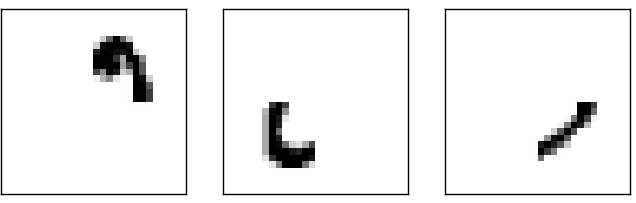
\includegraphics{http://neuralnetworksanddeeplearning.com/images/mnist_other_features.png}

First neuron in the hidden layer may detect just whether or not an image
like the above is present. If we had 4 outputs, then the first output
neuron would be trying to decide \textbf{what the most significant bit
of the digit} was. And there's \textbf{no easy way} to relate that most
significant bit to simple shapes like those shown above. However there
could be always such \textbf{structures with 4 neurons at the output so
that net were more efficient.} Now, with all that said, \textbf{this is
all just a heuristic.}

\subsection{Learning with gradient
descent}\label{learning-with-gradient-descent}

Now the first thing we'll need is a \textbf{data set} to learn from
so-called \textbf{training data set.} We'll use the
\href{http://yann.lecun.com/exdb/mnist/}{\textbf{MNIST data set}} which
contains \textbf{tens of thousands of scanned images of handwritten
digits, together with their correct classifications.} Images are the
same as used before.

\begin{figure}[htbp]
\centering
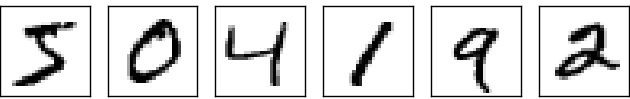
\includegraphics{http://neuralnetworksanddeeplearning.com/images/digits_separate.png}
\caption{MNIST}
\end{figure}

The MNIST data comes in \textbf{two parts.} The first part contains
\textbf{60,000 images to be used as training data.} These images are
scanned handwriting samples from 250 people, half of whom were US Census
Bureau employees, and half of whom were high school students. The
\textbf{images are grayscale and 28 by 28 pixels in size.} The second
part of the MNIST data set is \textbf{10,000 images to be used as test
data.} Again, these are 28 by 28 grayscale images. We'll \textbf{use the
test data to evaluate how well our neural network has learned to
recognize digits.} To make this a good test of performance, the
\textbf{test data was taken from a different set of 250 people than the
original training data} (albeit still a group split between Census
Bureau employees and high school students). This helps give us
confidence that our \textbf{system can recognize digits from people
whose writing it didn't see during training.}

We'll use the notation \$ x \$ to \textbf{denote a training input.}
It'll be convenient to regard each training input \$ x \$ as a \$ 28 *
28 = 784 \$ dimensional vector. \textbf{Each entry in the vector
represents the gray value for a single pixel in the image.} We'll denote
the corresponding desired output by \$ y = y(x) $, where $ y \$ is a
10-dimensional vector. For example, if a particular training image, \$ x
$, depicts a 6, then $ y(x)=(0,0,0,0,0,0,1,0,0,0) \^{} T \$ is the
desired output from the network. Note that \$ T \$ here is the
\textbf{transpose operation,} turning a row vector into an ordinary
(column) vector.

What we'd like is an algorithm which lets us \textbf{find weights and
biases} so that the output from the network \textbf{approximates} \$
y(x) \$ \textbf{for all training inputs} \$ x \$. To quantify how well
we're achieving this goal we define a \textbf{\emph{cost function.}}
Sometimes referred to as a \textbf{\emph{loss or objective function.}}

\begin{equation}
    C(w, \ b)\equiv\frac{1}{2n}\sum_x ||y(x) − a||^2
\end{equation}

Here, \$ w \$ denotes the \textbf{collection of all weights} in the
network, \$ b \$ \textbf{all the biases,} \$ n \$ is the \textbf{total
number of training inputs,} \$ a \$ is the \textbf{vector of outputs}
from the network when \$ x \$ is input, and the \textbf{sum is over all
training inputs, x.} Of course, the output \$ a \$ depends on \$ x, w \$
and \$ b $. The notation $ \textbar{}\textbar{}v\textbar{}\textbar{} \$
just denotes the \textbf{usual length function} for a vector \$ v
$. We'll call $ C \$ the \textbf{\emph{quadratic cost function}}; it's
also sometimes known as the \textbf{\emph{mean squared error or just
MSE.}} \$ C(w, ~b) \$ is \textbf{non-negative, since every term in the
sum is non-negative.} Furthermore, the cost \$ C(w, ~b) \$ precisely
when \$ y(x) \$ is approximately equal to the output, \$ a
$, for all training inputs, $ x
$. So our training algorithm has done a good job if it can **find weights and biases so that** $
C(w, ~b) \approx 0 $. By contrast, it's not doing so well when $ C(w,
~b) \$ is large - that would mean that \$ y(x) \$ is not close to the
output a for a large number of inputs. So the \textbf{aim of our
training algorithm will be to minimize the cost} \$ C(w, ~b) \$
\textbf{as a function of the weights and biases.}

Okay, let's suppose we're trying to minimize some function, \$ C(v)
$. This could be any real-valued function of many variables, $v = v1,
v2, \ldots{} \$

\begin{figure}[htbp]
\centering
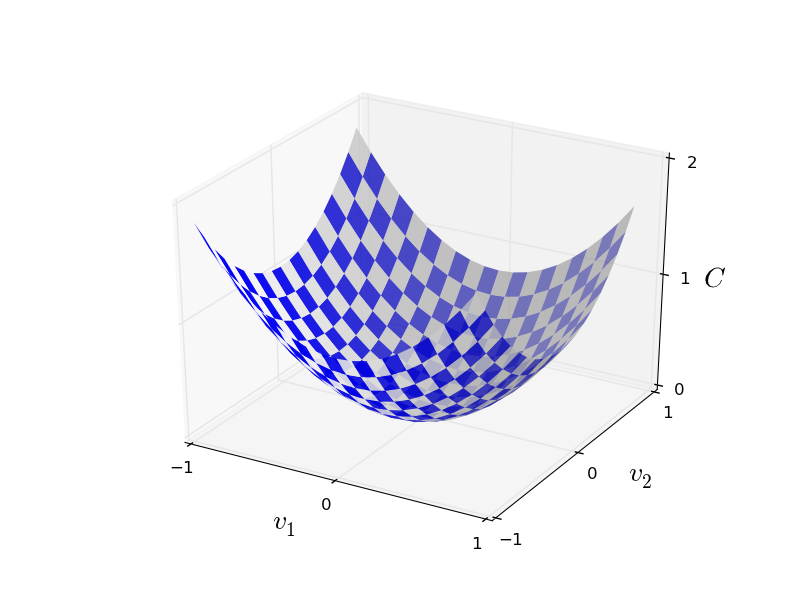
\includegraphics{http://neuralnetworksanddeeplearning.com/images/valley.png}
\caption{valley}
\end{figure}

What we'd like is to \textbf{find where} \$ C \$ \textbf{achieves its
global minimum.} One way of attacking the problem is to \textbf{use
calculus} to try to find the minimum analytically. With some luck that
might work when \$ C \$ is a function of just one or a few variables.
But it'll turn into a nightmare when we have many more variables. And
for neural networks we'll often want far more variables - the biggest
neural networks have cost functions which depend on \textbf{billions of
weights and biases} in an extremely complicated way. \textbf{Using
calculus to minimize that just won't work!} We start by thinking of our
function \textbf{as a kind of a valley.} And we imagine a ball rolling
down the slope of the valley. Our everyday experience tells us that the
ball will eventually roll to the bottom of the valley.

Let's think about what happens when we move the ball a small amount \$
\Delta v\_1 \$ in the \$ v\_1 \$ direction, and a small amount \$
\Delta v\_2 \$ in the \$ v\_2 \$ direction. Calculus tells us that C
changes as follows:

\begin{equation}
    \Delta C \approx \frac {\partial C}{\partial v_1} \Delta v_1 +
    \frac{\partial C}{\partial v_2} \Delta v_2
\end{equation}

We're going to find a way of choosing \$ \Delta v\_1 \$ and \$
\Delta v\_2 \$ so as to make \$ \Delta C \$ negative; i.e., we'll choose
them so the \textbf{ball is rolling down into the valley.} To figure out
how to make such a choice it helps to define \$ \Delta v \$ to be the
vector of changes in \$ v $, $ \Delta v \equiv (\Delta v\_1,
~\Delta v\_2)\^{}T $. We denote the gradient vector by $ \nabla C \$,
i.e.:

\begin{equation}
    \nabla C \equiv \left( \frac{\partial C}{\partial v_1}, \ \frac{\partial C} 
    {\partial v_2} \right)^T
\end{equation}

More generally, if \$ C \$ is function of \$ m \$ variables,

\begin{equation}
    \nabla C \equiv \left( \frac{\partial C}{\partial v_1}, 
    \frac{\partial C}{\partial v_2}, \ ..., \ \frac{\partial C} 
    {\partial v_m} \right)^T
\end{equation}

With these definitions, the expression (7) for \$ \Delta C \$ can be
rewritten as

\begin{equation}
    \Delta C \approx \nabla C ⋅ \Delta v
\end{equation}

In particular, suppose we choose,

\begin{equation}
    \Delta v = −\eta \nabla C
\end{equation}

where \$ \eta \$ \textbf{is a small, positive parameter (known as the
\emph{learning rate}).} Then Equation (9) becomes

\begin{equation}
     \Delta C \approx −\eta \nabla C ⋅ \nabla C = −\eta || \nabla C|| ^ 2
\end{equation}

This guarantees that \$ \Delta C \leq 0 $, i.e., $ C \$ \textbf{will
always decrease.} This is exactly the property we wanted! And so we'll
take Equation (10) to define the \textbf{``law of motion'' for the ball}
in our gradient descent algorithm. That is, we'll use Equation (10) to
compute a value for \$ \Delta v \$, then move the ball's position v by
that amount:

\begin{equation}
     v \to v' = v − \eta \nabla C
\end{equation}

Then we'll use this update rule again, to make another move. If we keep
doing this, over and over, we'll \textbf{keep decreasing \$ C \$ until -
we hope - we reach a global minimum.}

Summing up, the way the gradient descent algorithm works is to
repeatedly \textbf{compute the gradient} \$ \nabla C \$, \textbf{and
then to move in the opposite direction, ``falling down'' the slope of
the valley.}

To make gradient descent work correctly, we need to \textbf{choose the
learning rate} \$ \eta \$ \textbf{to be small enough that Equation (9)
is a good approximation.} If we don't, we might end up with \$ \Delta C
\textgreater{} 0
$, which obviously would not be good! At the same time, **we don't want** $
\eta \$ \textbf{to be too small, since that will make the changes} \$
\Delta v \$ \textbf{tiny, and thus the gradient descent algorithm will
work very slowly.}

Unfortunately, \textbf{this rule does not always work} - several things
can go wrong and \textbf{prevent gradient descent from finding the
global minimum} of \$ C \$, a point we'll return to explore in later
chapters. But, \textbf{in practice gradient descent often works
extremely well}, and in neural networks we'll find that it's a powerful
way of minimizing the cost function, and so helping the net learn.

How can we apply gradient descent to learn in a neural network? The idea
is to use gradient descent to find the weights \$ w\_k \$ and biases \$
b\_l \$ which minimize the cost in Equation (6). To see how this works,
let's restate the gradient descent update rule, with the weights and
biases replacing the variables \$ v\_j \$.

\begin{equation}
    w_k \to w_k' = w_k − \eta \frac{\partial C}{\partial w_k} \\
    b_l \to b_l′ = b_l − \eta \frac{\partial C}{\partial b_l}
\end{equation}

By repeatedly applying this update rule we can ``roll down the hill'',
and hopefully find a minimum of the cost function. In other words, this
is a rule which can be used to learn in a neural network.

Notice that this cost function has the form \$ C = \frac{1}{n}
\sum\emph{x C}x $, that is, it's an **average over costs** $ C\_x ≡
\frac{||y(x) − a|| ^ 2}{2} \$ for individual training examples. In
practice, to compute the gradient \$ \nabla C \$ we need to
\textbf{compute the gradients} \$ \nabla C\_x \$ \textbf{separately} for
each training input, \$ x $, and then average them, $ \nabla C =
\frac{1}{n} \sum\emph{x \nabla C}x \$. Unfortunately, when the number of
training inputs is very large this can \textbf{take a long time}, and
\textbf{learning thus occurs slowly.}

An idea called \textbf{\emph{stochastic gradient descent}} can be used
to \textbf{speed up learning}. The idea is to \textbf{estimate the
gradient} \$ \nabla C \$ by computing \$ \nabla C\_x \$ for a
\textbf{small sample of randomly chosen training inputs.} By
\textbf{averaging over this small sample} it turns out that we can
quickly get a \textbf{good estimate of the true gradient} \$ \nabla C
\$, and this \textbf{helps speed up gradient descent, and thus
learning.}

To make these ideas more precise, stochastic gradient descent works by
\textbf{randomly picking out a small number} \$ m \$ \textbf{of randomly
chosen training inputs.} We'll label those random training inputs \$
X\_1, X\_2,\ldots{}, X\_m \$ and refer to them as a
\textbf{\emph{mini-batch.}}

It's much \textbf{easier to sample a small mini-batch than it is to
apply gradient descent to the full batch.} For example, if we have a
training set of size n=60,000, as in MNIST, and choose a mini-batch size
of (say) m=10, this means we'll get a factor of \textbf{6,000 speedup}
in estimating the gradient! Of course, the estimate won't be perfect -
there will be statistical fluctuations - but it doesn't need to be
perfect: all we really care about is moving in a general direction that
will help decrease C, and that means we don't need an exact computation
of the gradient. In practice, \textbf{stochastic gradient descent is a
commonly used and powerful technique for learning in neural networks.}

\end{document}
